\documentclass[nooutcomes]{ximera}

\graphicspath{
  {./}
  {1-1QuantitativeReasoning/}
  {1-2RelationsAndGraphs/}
  {1-3ChangingInTandem/}
  {2-1LinearEquations/}
  {2-2LinearModeling/}
  {2-3ExponentialModeling/}
  {3-1WhatIsAFunction/}
  {3-2FunctionProperties/}
  {3-3AverageRatesOfChange/}
  {4-1BuildingNewFunctions/}
  {4-2Polynomials/}
  {5-1RationalFunctions/}
   {5-2ExponentialFunctions/}
  {6-1Domain/}
  {6-2Range/}
  {6-3CompositionOfFunctions/}
  {6-4FunctionTransformations/}
  {7-1ZerosOfFunctions/}
  {7-XZerosOfPolynomials/}
  {7-2ZerosOfFamousFunctions/}
  {8-1SystemsOfEquations/}
  {6-5FunctionTransformationsProject/}
  {1-1QuantitativeReasoning/exercises/}
  {1-2RelationsAndGraphs/exercises/}
  {../1-3ChangingInTandem/exercises/}
  {../2-1LinearEquations/exercises/}
  {../2-2LinearModeling/exercises/}
  {../2-3ExponentialModeling/exercises/}
  {../3-1WhatIsAFunction/exercises/}
  {../3-2FunctionProperties/exercises/}
  {../3-3AverageRatesOfChange/exercises/}
  {../5-2ExponentialFunctions/exercises/}
  {../4-1BuildingNewFunctions/exercises/}
  {../4-2Polynomials/exercises/}
  {../5-1RationalFunctions/exercises/}
  {../6-1Domain/exercises/}
  {../6-2Range/exercises/}
  {../6-3CompositionOfFunctions/exercises/}
  {../7-1ZerosOfFunctions/exercises/}
  {../7-XZerosOfPolynomials/exercises/}
  {../7-2ZerosOfFamousFunctions/exercises/}
  {../6-4FunctionTransformations/exercises/}
  {../8-1SystemsOfEquations/exercises/}
  {../6-3FunctionTransformationsProject/exercises/}
}

\DeclareGraphicsExtensions{.pdf,.png,.jpg,.eps}

\newcommand{\mooculus}{\textsf{\textbf{MOOC}\textnormal{\textsf{ULUS}}}}

\usepackage[makeroom]{cancel} %% for strike outs

\ifxake
\else
\usepackage[most]{tcolorbox}
\fi


%\typeout{************************************************}
%\typeout{New Environments}
%\typeout{************************************************}

%% to fix for web can be removed when deployed offically with ximera2
\let\image\relax\let\endimage\relax
\NewEnviron{image}{% 
  \begin{center}\BODY\end{center}% center
}



\NewEnviron{folder}{
      \addcontentsline{toc}{section}{\textbf{\BODY}}
}

\ifxake
\let\summary\relax
\let\endsummary\relax
\newtheorem*{summary}{Summary}
\newtheorem*{callout}{Callout}
\newtheorem*{overview}{Overview}
\newtheorem*{objectives}{Objectives}
\newtheorem*{motivatingQuestions}{Motivating Questions}
\newtheorem*{MM}{Metacognitive Moment}
      
%% NEEDED FOR XIMERA 2
%\ximerizedEnvironment{summary}
%\ximerizedEnvironment{callout}
%\ximerizedEnvironment{overview} 
%\ximerizedEnvironment{objectives}
%\ximerizedEnvironment{motivatingQuestions}
%\ximerizedEnvironment{MM}
\else
%% CALLOUT
\NewEnviron{callout}{
  \begin{tcolorbox}[colback=blue!5, breakable,pad at break*=1mm]
      \BODY
  \end{tcolorbox}
}
%% MOTIVATING QUESTIONS
\NewEnviron{motivatingQuestions}{
  \begin{tcolorbox}[ breakable,pad at break*=1mm]
    \textbf{\Large Motivating Questions}\hfill
    %\begin{itemize}[label=\textbullet]
      \BODY
    %\end{itemize}
  \end{tcolorbox}
}
%% OBJECTIVES
\NewEnviron{objectives}{  
    \vspace{.5in}
      %\begin{tcolorbox}[colback=orange!5, breakable,pad at break*=1mm]
    \textbf{\Large Learning Objectives}
    \begin{itemize}[label=\textbullet]
      \BODY
    \end{itemize}
    %\end{tcolorbox}
}
%% DEFINITION
\let\definition\relax
\let\enddefinition\relax
\NewEnviron{definition}{
  \begin{tcolorbox}[ breakable,pad at break*=1mm]
    \noindent\textbf{Definition}~
      \BODY
  \end{tcolorbox}
}
%% OVERVIEW
\let\overview\relax
\let\overview\relax
\NewEnviron{overview}{
  \begin{tcolorbox}[ breakable,pad at break*=1mm]
    \textbf{\Large Overview}
    %\begin{itemize}[label=\textbullet] %% breaks Xake
      \BODY
    %\end{itemize}
  \end{tcolorbox}
}
%% SUMMARY
\let\summary\relax
\let\endsummary\relax
\NewEnviron{summary}{
  \begin{tcolorbox}[ breakable,pad at break*=1mm]
    \textbf{\Large Summary}
    %\begin{itemize}[label=\textbullet] %% breaks Xake
      \BODY
    %\end{itemize}
  \end{tcolorbox}
}
%% REMARK
\let\remark\relax
\let\endremark\relax
\NewEnviron{remark}{
  \begin{tcolorbox}[colback=green!5, breakable,pad at break*=1mm]
    \noindent\textbf{Remark}~
      \BODY
  \end{tcolorbox}
}
%% EXPLANATION
\let\explanation\relax
\let\endexplanation\relax
\NewEnviron{explanation}{
    \normalfont
    \noindent\textbf{Explanation}~
      \BODY
}
%% EXPLORATION
\let\exploration\relax
\let\endexploration\relax
\NewEnviron{exploration}{
  \begin{tcolorbox}[colback=yellow!10, breakable,pad at break*=1mm]
    \noindent\textbf{Exploration}~
      \BODY
  \end{tcolorbox}
}
%% METACOGNITIVE MOMENTS
\let\MM\relax
\let\endMM\relax
\NewEnviron{MM}{
  \begin{tcolorbox}[colback=pink!15, breakable,pad at break*=1mm]
    \noindent\textbf{Metacognitive Moment}~
      \BODY
  \end{tcolorbox}
}


\fi





%Notes on what envirnoment to use:  Example with Explanation in text; if they are supposed to answer- Problem; no answer - Exploration


%\typeout{************************************************}
%% Header and footers
%\typeout{************************************************}

\newcommand{\licenseAcknowledgement}{Licensed under Creative Commons 4.0}
\newcommand{\licenseAPC}{\renewcommand{\licenseAcknowledgement}{\textbf{Acknowledgements:} Active Prelude to Calculus (https://activecalculus.org/prelude) }}
\newcommand{\licenseSZ}{\renewcommand{\licenseAcknowledgement}{\textbf{Acknowledgements:} Stitz Zeager Open Source Mathematics (https://www.stitz-zeager.com/) }}
\newcommand{\licenseAPCSZ}{\renewcommand{\licenseAcknowledgement}{\textbf{Acknowledgements:} Active Prelude to Calculus (https://activecalculus.org/prelude) and Stitz Zeager Open Source Mathematics (https://www.stitz-zeager.com/) }}
\newcommand{\licenseORCCA}{\renewcommand{\licenseAcknowledgement}{\textbf{Acknowledgements:}Original source material, products with readable and accessible
math content, and other information freely available at pcc.edu/orcca.}}
\newcommand{\licenseY}{\renewcommand{\licenseAcknowledgement}{\textbf{Acknowledgements:} Yoshiwara Books (https://yoshiwarabooks.org/)}}
\newcommand{\licenseOS}{\renewcommand{\licenseAcknowledgement}{\textbf{Acknowledgements:} OpenStax College Algebra (https://openstax.org/details/books/college-algebra)}}
\newcommand{\licenseAPCSZCSCC}{\renewcommand{\licenseAcknowledgement}{\textbf{Acknowledgements:} Active Prelude to Calculus (https://activecalculus.org/prelude), Stitz Zeager Open Source Mathematics (https://www.stitz-zeager.com/), CSCC PreCalculus and Calculus texts (https://ximera.osu.edu/csccmathematics)}}

\ifxake\else %% do nothing on the website
\usepackage{fancyhdr}
\pagestyle{fancy}
\fancyhf{}
\fancyhead[R]{\sectionmark}
\fancyfoot[L]{\thepage}
\fancyfoot[C]{\licenseAcknowledgement}
\renewcommand{\headrulewidth}{0pt}
\renewcommand{\footrulewidth}{0pt}
\fi

%%%%%%%%%%%%%%%%



%\typeout{************************************************}
%\typeout{Table of Contents}
%\typeout{************************************************}


%% Edit this to change the font style
\newcommand{\sectionHeadStyle}{\sffamily\bfseries}


\makeatletter

%% part uses arabic numerals
\renewcommand*\thepart{\arabic{part}}


\ifxake\else
\renewcommand\chapterstyle{%
  \def\maketitle{%
    \addtocounter{titlenumber}{1}%
    \pagestyle{fancy}
    \phantomsection
    \addcontentsline{toc}{section}{\textbf{\thepart.\thetitlenumber\hspace{1em}\@title}}%
                    {\flushleft\small\sectionHeadStyle\@pretitle\par\vspace{-1.5em}}%
                    {\flushleft\LARGE\sectionHeadStyle\thepart.\thetitlenumber\hspace{1em}\@title \par }%
                    {\setcounter{problem}{0}\setcounter{sectiontitlenumber}{0}}%
                    \par}}





\renewcommand\sectionstyle{%
  \def\maketitle{%
    \addtocounter{sectiontitlenumber}{1}
    \pagestyle{fancy}
    \phantomsection
    \addcontentsline{toc}{subsection}{\thepart.\thetitlenumber.\thesectiontitlenumber\hspace{1em}\@title}%
    {\flushleft\small\sectionHeadStyle\@pretitle\par\vspace{-1.5em}}%
    {\flushleft\Large\sectionHeadStyle\thepart.\thetitlenumber.\thesectiontitlenumber\hspace{1em}\@title \par}%
    %{\setcounter{subsectiontitlenumber}{0}}%
    \par}}



\renewcommand\section{\@startsection{paragraph}{10}{\z@}%
                                     {-3.25ex\@plus -1ex \@minus -.2ex}%
                                     {1.5ex \@plus .2ex}%
                                     {\normalfont\large\sectionHeadStyle}}
\renewcommand\subsection{\@startsection{subparagraph}{10}{\z@}%
                                    {3.25ex \@plus1ex \@minus.2ex}%
                                    {-1em}%
                                    {\normalfont\normalsize\sectionHeadStyle}}

\fi

%% redefine Part
\renewcommand\part{%
   {\setcounter{titlenumber}{0}}
  \if@openright
    \cleardoublepage
  \else
    \clearpage
  \fi
  \thispagestyle{plain}%
  \if@twocolumn
    \onecolumn
    \@tempswatrue
  \else
    \@tempswafalse
  \fi
  \null\vfil
  \secdef\@part\@spart}

\def\@part[#1]#2{%
    \ifnum \c@secnumdepth >-2\relax
      \refstepcounter{part}%
      \addcontentsline{toc}{part}{\thepart\hspace{1em}#1}%
    \else
      \addcontentsline{toc}{part}{#1}%
    \fi
    \markboth{}{}%
    {\centering
     \interlinepenalty \@M
     \normalfont
     \ifnum \c@secnumdepth >-2\relax
       \huge\sffamily\bfseries \partname\nobreakspace\thepart
       \par
       \vskip 20\p@
     \fi
     \Huge \bfseries #2\par}%
    \@endpart}
\def\@spart#1{%
    {\centering
     \interlinepenalty \@M
     \normalfont
     \Huge \bfseries #1\par}%
    \@endpart}
\def\@endpart{\vfil\newpage
              \if@twoside
               \if@openright
                \null
                \thispagestyle{empty}%
                \newpage
               \fi
              \fi
              \if@tempswa
                \twocolumn
                \fi}



\makeatother





%\typeout{************************************************}
%\typeout{Stuff from Ximera}
%\typeout{************************************************}



\usepackage{array}  %% This is for typesetting long division
\setlength{\extrarowheight}{+.1cm}
\newdimen\digitwidth
\settowidth\digitwidth{9}
\def\divrule#1#2{
\noalign{\moveright#1\digitwidth
\vbox{\hrule width#2\digitwidth}}}





\newcommand{\RR}{\mathbb R}
\newcommand{\R}{\mathbb R}
\newcommand{\N}{\mathbb N}
\newcommand{\Z}{\mathbb Z}

\newcommand{\sagemath}{\textsf{SageMath}}


\def\d{\,d}
%\renewcommand{\d}{\mathop{}\!d}
\newcommand{\dd}[2][]{\frac{\d #1}{\d #2}}
\newcommand{\pp}[2][]{\frac{\partial #1}{\partial #2}}
\renewcommand{\l}{\ell}
\newcommand{\ddx}{\frac{d}{\d x}}



%\newcommand{\unit}{\,\mathrm}
\newcommand{\unit}{\mathop{}\!\mathrm}
\newcommand{\eval}[1]{\bigg[ #1 \bigg]}
\newcommand{\seq}[1]{\left( #1 \right)}
\renewcommand{\epsilon}{\varepsilon}
\renewcommand{\phi}{\varphi}


\renewcommand{\iff}{\Leftrightarrow}

\DeclareMathOperator{\arccot}{arccot}
\DeclareMathOperator{\arcsec}{arcsec}
\DeclareMathOperator{\arccsc}{arccsc}
\DeclareMathOperator{\sign}{sign}


%\DeclareMathOperator{\divergence}{divergence}
%\DeclareMathOperator{\curl}[1]{\grad\cross #1}
\newcommand{\lto}{\mathop{\longrightarrow\,}\limits}

\renewcommand{\bar}{\overline}

\colorlet{textColor}{black}
\colorlet{background}{white}
\colorlet{penColor}{blue!50!black} % Color of a curve in a plot
\colorlet{penColor2}{red!50!black}% Color of a curve in a plot
\colorlet{penColor3}{red!50!blue} % Color of a curve in a plot
\colorlet{penColor4}{green!50!black} % Color of a curve in a plot
\colorlet{penColor5}{orange!80!black} % Color of a curve in a plot
\colorlet{penColor6}{yellow!70!black} % Color of a curve in a plot
\colorlet{fill1}{penColor!20} % Color of fill in a plot
\colorlet{fill2}{penColor2!20} % Color of fill in a plot
\colorlet{fillp}{fill1} % Color of positive area
\colorlet{filln}{penColor2!20} % Color of negative area
\colorlet{fill3}{penColor3!20} % Fill
\colorlet{fill4}{penColor4!20} % Fill
\colorlet{fill5}{penColor5!20} % Fill
\colorlet{gridColor}{gray!50} % Color of grid in a plot

\newcommand{\surfaceColor}{violet}
\newcommand{\surfaceColorTwo}{redyellow}
\newcommand{\sliceColor}{greenyellow}




\pgfmathdeclarefunction{gauss}{2}{% gives gaussian
  \pgfmathparse{1/(#2*sqrt(2*pi))*exp(-((x-#1)^2)/(2*#2^2))}%
}





%\typeout{************************************************}
%\typeout{ORCCA Preamble.Tex}
%\typeout{************************************************}


%% \usepackage{geometry}
%% \geometry{letterpaper,total={408pt,9.0in}}
%% Custom Page Layout Adjustments (use latex.geometry)
%% \usepackage{amsmath,amssymb}
%% \usepackage{pgfplots}
\usepackage{pifont}                                         %needed for symbols, s.a. airplane symbol
\usetikzlibrary{positioning,fit,backgrounds}                %needed for nested diagrams
\usetikzlibrary{calc,trees,positioning,arrows,fit,shapes}   %needed for set diagrams
\usetikzlibrary{decorations.text}                           %needed for text following a curve
\usetikzlibrary{arrows,arrows.meta}                         %needed for open/closed intervals
\usetikzlibrary{positioning,3d,shapes.geometric}            %needed for 3d number sets tower

%% NEEDED FOR XIMERA 1
%\usetkzobj{all}       %NO LONGER VALID
%%%%%%%%%%%%%%

\usepackage{tikz-3dplot}
\usepackage{tkz-euclide}                     %needed for triangle diagrams
\usepgfplotslibrary{fillbetween}                            %shade regions of a plot
\usetikzlibrary{shadows}                                    %function diagrams
\usetikzlibrary{positioning}                                %function diagrams
\usetikzlibrary{shapes}                                     %function diagrams
%%% global colors from https://www.pcc.edu/web-services/style-guide/basics/color/ %%%
\definecolor{ruby}{HTML}{9E0C0F}
\definecolor{turquoise}{HTML}{008099}
\definecolor{emerald}{HTML}{1c8464}
\definecolor{amber}{HTML}{c7502a}
\definecolor{amethyst}{HTML}{70485b}
\definecolor{sapphire}{HTML}{263c53}
\colorlet{firstcolor}{sapphire}
\colorlet{secondcolor}{turquoise}
\colorlet{thirdcolor}{emerald}
\colorlet{fourthcolor}{amber}
\colorlet{fifthcolor}{amethyst}
\colorlet{sixthcolor}{ruby}
\colorlet{highlightcolor}{green!50!black}
\colorlet{graphbackground}{white}
\colorlet{wood}{brown!60!white}
%%% curve, dot, and graph custom styles %%%
\pgfplotsset{firstcurve/.style      = {color=firstcolor,  mark=none, line width=1pt, {Kite}-{Kite}, solid}}
\pgfplotsset{secondcurve/.style     = {color=secondcolor, mark=none, line width=1pt, {Kite}-{Kite}, solid}}
\pgfplotsset{thirdcurve/.style      = {color=thirdcolor,  mark=none, line width=1pt, {Kite}-{Kite}, solid}}
\pgfplotsset{fourthcurve/.style     = {color=fourthcolor, mark=none, line width=1pt, {Kite}-{Kite}, solid}}
\pgfplotsset{fifthcurve/.style      = {color=fifthcolor,  mark=none, line width=1pt, {Kite}-{Kite}, solid}}
\pgfplotsset{highlightcurve/.style  = {color=highlightcolor,  mark=none, line width=5pt, -, opacity=0.3}}   % thick, opaque curve for highlighting
\pgfplotsset{asymptote/.style       = {color=gray, mark=none, line width=1pt, <->, dashed}}
\pgfplotsset{symmetryaxis/.style    = {color=gray, mark=none, line width=1pt, <->, dashed}}
\pgfplotsset{guideline/.style       = {color=gray, mark=none, line width=1pt, -}}
\tikzset{guideline/.style           = {color=gray, mark=none, line width=1pt, -}}
\pgfplotsset{altitude/.style        = {dashed, color=gray, thick, mark=none, -}}
\tikzset{altitude/.style            = {dashed, color=gray, thick, mark=none, -}}
\pgfplotsset{radius/.style          = {dashed, thick, mark=none, -}}
\tikzset{radius/.style              = {dashed, thick, mark=none, -}}
\pgfplotsset{rightangle/.style      = {color=gray, mark=none, -}}
\tikzset{rightangle/.style          = {color=gray, mark=none, -}}
\pgfplotsset{closedboundary/.style  = {color=black, mark=none, line width=1pt, {Kite}-{Kite},solid}}
\tikzset{closedboundary/.style      = {color=black, mark=none, line width=1pt, {Kite}-{Kite},solid}}
\pgfplotsset{openboundary/.style    = {color=black, mark=none, line width=1pt, {Kite}-{Kite},dashed}}
\tikzset{openboundary/.style        = {color=black, mark=none, line width=1pt, {Kite}-{Kite},dashed}}
\tikzset{verticallinetest/.style    = {color=gray, mark=none, line width=1pt, <->,dashed}}
\pgfplotsset{soliddot/.style        = {color=firstcolor,  mark=*, only marks}}
\pgfplotsset{hollowdot/.style       = {color=firstcolor,  mark=*, only marks, fill=graphbackground}}
\pgfplotsset{blankgraph/.style      = {xmin=-10, xmax=10,
                                        ymin=-10, ymax=10,
                                        axis line style={-, draw opacity=0 },
                                        axis lines=box,
                                        major tick length=0mm,
                                        xtick={-10,-9,...,10},
                                        ytick={-10,-9,...,10},
                                        grid=major,
                                        grid style={solid,gray!20},
                                        xticklabels={,,},
                                        yticklabels={,,},
                                        minor xtick=,
                                        minor ytick=,
                                        xlabel={},ylabel={},
                                        width=0.75\textwidth,
                                      }
            }
\pgfplotsset{numberline/.style      = {xmin=-10,xmax=10,
                                        minor xtick={-11,-10,...,11},
                                        xtick={-10,-5,...,10},
                                        every tick/.append style={thick},
                                        axis y line=none,
                                        y=15pt,
                                        axis lines=middle,
                                        enlarge x limits,
                                        grid=none,
                                        clip=false,
                                        axis background/.style={},
                                        after end axis/.code={
                                          \path (axis cs:0,0)
                                          node [anchor=north,yshift=-0.075cm] {\footnotesize 0};
                                        },
                                        every axis x label/.style={at={(current axis.right of origin)},anchor=north},
                                      }
            }
\pgfplotsset{openinterval/.style={color=firstcolor,mark=none,ultra thick,{Parenthesis}-{Parenthesis}}}
\pgfplotsset{openclosedinterval/.style={color=firstcolor,mark=none,ultra thick,{Parenthesis}-{Bracket}}}
\pgfplotsset{closedinterval/.style={color=firstcolor,mark=none,ultra thick,{Bracket}-{Bracket}}}
\pgfplotsset{closedopeninterval/.style={color=firstcolor,mark=none,ultra thick,{Bracket}-{Parenthesis}}}
\pgfplotsset{infiniteopeninterval/.style={color=firstcolor,mark=none,ultra thick,{Kite}-{Parenthesis}}}
\pgfplotsset{openinfiniteinterval/.style={color=firstcolor,mark=none,ultra thick,{Parenthesis}-{Kite}}}
\pgfplotsset{infiniteclosedinterval/.style={color=firstcolor,mark=none,ultra thick,{Kite}-{Bracket}}}
\pgfplotsset{closedinfiniteinterval/.style={color=firstcolor,mark=none,ultra thick,{Bracket}-{Kite}}}
\pgfplotsset{infiniteinterval/.style={color=firstcolor,mark=none,ultra thick,{Kite}-{Kite}}}
\pgfplotsset{interval/.style= {ultra thick, -}}
%%% cycle list of plot styles for graphs with multiple plots %%%
\pgfplotscreateplotcyclelist{pccstylelist}{%
  firstcurve\\%
  secondcurve\\%
  thirdcurve\\%
  fourthcurve\\%
  fifthcurve\\%
}
%%% default plot settings %%%
\pgfplotsset{every axis/.append style={
  axis x line=middle,    % put the x axis in the middle
  axis y line=middle,    % put the y axis in the middle
  axis line style={<->}, % arrows on the axis
  scaled ticks=false,
  tick label style={/pgf/number format/fixed},
  xlabel={$x$},          % default put x on x-axis
  ylabel={$y$},          % default put y on y-axis
  xmin = -7,xmax = 7,    % most graphs have this window
  ymin = -7,ymax = 7,    % most graphs have this window
  domain = -7:7,
  xtick = {-6,-4,...,6}, % label these ticks
  ytick = {-6,-4,...,6}, % label these ticks
  yticklabel style={inner sep=0.333ex},
  minor xtick = {-7,-6,...,7}, % include these ticks, some without label
  minor ytick = {-7,-6,...,7}, % include these ticks, some without label
  scale only axis,       % don't consider axis and tick labels for width and height calculation
  cycle list name=pccstylelist,
  tick label style={font=\footnotesize},
  legend cell align=left,
  grid = both,
  grid style = {solid,gray!20},
  axis background/.style={fill=graphbackground},
}}
\pgfplotsset{framed/.style={axis background/.style ={draw=gray}}}
%\pgfplotsset{framed/.style={axis background/.style ={draw=gray,fill=graphbackground,rounded corners=3ex}}}
%%% other tikz (not pgfplots) settings %%%
%\tikzset{axisnode/.style={font=\scriptsize,text=black}}
\tikzset{>=stealth}
%%% for nested diagram in types of numbers section %%%
\newcommand\drawnestedsets[4]{
  \def\position{#1}             % initial position
  \def\nbsets{#2}               % number of sets
  \def\listofnestedsets{#3}     % list of sets
  \def\reversedlistofcolors{#4} % reversed list of colors
  % position and draw labels of sets
  \coordinate (circle-0) at (#1);
  \coordinate (set-0) at (#1);
  \foreach \set [count=\c] in \listofnestedsets {
    \pgfmathtruncatemacro{\cminusone}{\c - 1}
    % label of current set (below previous nested set)
    \node[below=3pt of circle-\cminusone,inner sep=0]
    (set-\c) {\set};
    % current set (fit current label and previous set)
    \node[circle,inner sep=0,fit=(circle-\cminusone)(set-\c)]
    (circle-\c) {};
  }
  % draw and fill sets in reverse order
  \begin{scope}[on background layer]
    \foreach \col[count=\c] in \reversedlistofcolors {
      \pgfmathtruncatemacro{\invc}{\nbsets-\c}
      \pgfmathtruncatemacro{\invcplusone}{\invc+1}
      \node[circle,draw,fill=\col,inner sep=0,
      fit=(circle-\invc)(set-\invcplusone)] {};
    }
  \end{scope}
  }
\ifdefined\tikzset
\tikzset{ampersand replacement = \amp}
\fi
\newcommand{\abs}[1]{\left\lvert#1\right\rvert}
%\newcommand{\point}[2]{\left(#1,#2\right)}
\newcommand{\highlight}[1]{\definecolor{sapphire}{RGB}{59,90,125} {\color{sapphire}{{#1}}}}
\newcommand{\firsthighlight}[1]{\definecolor{sapphire}{RGB}{59,90,125} {\color{sapphire}{{#1}}}}
\newcommand{\secondhighlight}[1]{\definecolor{emerald}{RGB}{20,97,75} {\color{emerald}{{#1}}}}
\newcommand{\unhighlight}[1]{{\color{black}{{#1}}}}
\newcommand{\lowlight}[1]{{\color{lightgray}{#1}}}
\newcommand{\attention}[1]{\mathord{\overset{\downarrow}{#1}}}
\newcommand{\nextoperation}[1]{\mathord{\boxed{#1}}}
\newcommand{\substitute}[1]{{\color{blue}{{#1}}}}
\newcommand{\pinover}[2]{\overset{\overset{\mathrm{\ #2\ }}{|}}{\strut #1 \strut}}
\newcommand{\addright}[1]{{\color{blue}{{{}+#1}}}}
\newcommand{\addleft}[1]{{\color{blue}{{#1+{}}}}}
\newcommand{\subtractright}[1]{{\color{blue}{{{}-#1}}}}
\newcommand{\multiplyright}[2][\cdot]{{\color{blue}{{{}#1#2}}}}
\newcommand{\multiplyleft}[2][\cdot]{{\color{blue}{{#2#1{}}}}}
\newcommand{\divideunder}[2]{\frac{#1}{{\color{blue}{{#2}}}}}
\newcommand{\divideright}[1]{{\color{blue}{{{}\div#1}}}}
\newcommand{\negate}[1]{{\color{blue}{{-}}}\left(#1\right)}
\newcommand{\cancelhighlight}[1]{\definecolor{sapphire}{RGB}{59,90,125}{\color{sapphire}{{\cancel{#1}}}}}
\newcommand{\secondcancelhighlight}[1]{\definecolor{emerald}{RGB}{20,97,75}{\color{emerald}{{\bcancel{#1}}}}}
\newcommand{\thirdcancelhighlight}[1]{\definecolor{amethyst}{HTML}{70485b}{\color{amethyst}{{\xcancel{#1}}}}}
\newcommand{\lt}{<} %% Bart: WHY?
\newcommand{\gt}{>} %% Bart: WHY?
\newcommand{\amp}{&} %% Bart: WHY?


%%% These commands break Xake
%% \newcommand{\apple}{\text{🍎}}
%% \newcommand{\banana}{\text{🍌}}
%% \newcommand{\pear}{\text{🍐}}
%% \newcommand{\cat}{\text{🐱}}
%% \newcommand{\dog}{\text{🐶}}

\newcommand{\apple}{PICTURE OF APPLE}
\newcommand{\banana}{PICTURE OF BANANA}
\newcommand{\pear}{PICTURE OF PEAR}
\newcommand{\cat}{PICTURE OF CAT}
\newcommand{\dog}{PICTURE OF DOG}


%%%%% INDEX STUFF
\newcommand{\dfn}[1]{\textbf{#1}\index{#1}}
\usepackage{imakeidx}
\makeindex[intoc]
\makeatletter
\gdef\ttl@savemark{\sectionmark{}}
\makeatother












 % for drawing cube in Optimization problem
\usetikzlibrary{quotes,arrows.meta}
\tikzset{
  annotated cuboid/.pic={
    \tikzset{%
      every edge quotes/.append style={midway, auto},
      /cuboid/.cd,
      #1
    }
    \draw [every edge/.append style={pic actions, densely dashed, opacity=.5}, pic actions]
    (0,0,0) coordinate (o) -- ++(-\cubescale*\cubex,0,0) coordinate (a) -- ++(0,-\cubescale*\cubey,0) coordinate (b) edge coordinate [pos=1] (g) ++(0,0,-\cubescale*\cubez)  -- ++(\cubescale*\cubex,0,0) coordinate (c) -- cycle
    (o) -- ++(0,0,-\cubescale*\cubez) coordinate (d) -- ++(0,-\cubescale*\cubey,0) coordinate (e) edge (g) -- (c) -- cycle
    (o) -- (a) -- ++(0,0,-\cubescale*\cubez) coordinate (f) edge (g) -- (d) -- cycle;
    \path [every edge/.append style={pic actions, |-|}]
    (b) +(0,-5pt) coordinate (b1) edge ["x"'] (b1 -| c)
    (b) +(-5pt,0) coordinate (b2) edge ["y"] (b2 |- a)
    (c) +(3.5pt,-3.5pt) coordinate (c2) edge ["x"'] ([xshift=3.5pt,yshift=-3.5pt]e)
    ;
  },
  /cuboid/.search also={/tikz},
  /cuboid/.cd,
  width/.store in=\cubex,
  height/.store in=\cubey,
  depth/.store in=\cubez,
  units/.store in=\cubeunits,
  scale/.store in=\cubescale,
  width=10,
  height=10,
  depth=10,
  units=cm,
  scale=.1,
}

\author{Kenneth Berglund}
\license{Creative Commons Attribution-ShareAlike 4.0 International License}
\acknowledgement{https://www.stitz-zeager.com/szca07042013.pdf}

\title{From Systems to Solutions}

\begin{document}
\begin{abstract}
  
\end{abstract}
\maketitle

\begin{motivatingQuestions}
\item What is a system of equations?
\item What is a solution to a system?
\item How can we solve systems of equations using graphs?
\end{motivatingQuestions}

%\typeout{************************************************}
%\typeout{Introduction}
%\typeout{************************************************}
\section{Introduction}

We have already seen many techniques for solving equations. Until now, however, we have only solved equations of the form $f(x) = 0$ for the variable $x$. In this section, we will consider equations with more than one variable and discuss how to solve them.

Consider a peculiar grocery store where the prices of all the items for sale are not listed, and you only find out the total cost of your purchase. Say you buy 6 mangos and 3 bananas, and your total cost is 9 dollars. Assume all the mangos cost the same amount and all the bananas cost the same amount. Without making any more purchases, is it possible find out how much a mango and a banana cost on their own? 

Let's create an equation to describe this situation. Let $x$ be a variable representing the cost of a mango, and let $y$ be a variable representing the cost of a banana. Then, the equation
$$
6x + 3y = 9
$$
represents that buying 6 mangos at a cost of $x$ dollars and 3 bananas at a cost of $y$ dollars yields a total cost of 9 dollars. 

You might have noticed that plugging $x = 1$ and $y = 1$ into the equation gives us a true statement, so you might conclude that mangos and bananas both cost 1 dollar. However, notice that plugging $x = 1.20$ and $y = 0.60$ into the equation also gives us a true statement, so it's also possible that mangos cost \$1.20 and bananas cost \$0.60. Even more worrying is that $x = 0$ and $y = 3$ also gives us a solution to the equation: is this store peculiar enough to be giving away mangos for free and charging \$3 per banana?

Examining the equation we set up can give us more insight. Let's rearrange the equation to solve for $y$ in terms of $x$:
\begin{align*}
6x + 3y & = 9 \\
3y & = 9 - 6x \\
y & = 3 - 2x.
\end{align*}
Now it becomes clearer what's going on. Whatever $x$ is, we can find a value of $y$ that satisfies our original equation. No matter the cost of a single mango, there's a way to price the bananas so that our equation is true! This means it's impossible to find the price of a single mango or a single banana with the information you've been given. We need more data!

%%\typeout{************************************************}
%%\typeout{Systems of linear equations}
%%\typeout{************************************************}
\section{Systems of linear equations}

In order to collect more information, you go back to the store and buy 2 mangos and 2 banana for a total cost of \$3.20. This can be modeled by the equation 
$$
2x + 2y = 3.2.
$$
Keep in mind that this $x$ and $y$ are the same $x$ and $y$ from before, so in order to find the cost of a mango and a banana, we must find $x$ and $y$ that satisfy both equations
$$
\begin{cases}
6x + 3y = 9 \\
2x + 2y = 3.2
\end{cases}
$$
at the same time. This coupling of two (or more) linear equations is called a \emph{system of linear equations}.

\begin{definition}
A \index{linear equation ! of two variables}\index{linear equation of two variables}\dfn{linear equation of two variables} is an equation of the form
$$
a_1 x + a_2 y = c,
$$
where $a_1$, $a_2$, and $c$ are real numbers and at least one of $a_1$ and 	$a_2$ is nonzero.

A \index{system of linear equations ! of two variables}\dfn{system of linear equations of two variables} is a collection of two or more linear equations of two variables.

We say a \dfn{solution} to a system of linear equations of two variables is a point $(x, y)$ satisfying all equations in the system. 
\end{definition}

The key to identifying linear equations is to note that the variables involved are to the first power and that the coefficients of the variables are numbers. Some examples of equations which are non-linear are $x^2+y = 1$, $xy = 5$ and $e^{2x} + \ln(y) = 1$. Note that we can still have systems of non-linear equations, but they can be much more difficult to solve. 

%%\typeout{************************************************}
%%\typeout{Finding solutions graphically}
%%\typeout{************************************************}
\section{Finding solutions graphically}
Let's return to our example from earlier and try to find a solution to the system of linear equation:
$$
\begin{cases}
6x + 3y = 9 \\
2x + 2y = 3.2
\end{cases}.
$$
We want to find $x$ and $y$ satisfying both equations in the system. If $x$ and $y$ satisfy $6x + 3y = 9$, then the point $(x, y)$ lies on the graph of $6x + 3y = 9$. Similarly, if $x$ and $y$ satisfy $2x + 2y = 3.2$, then the point $(x, y)$ lies on the graph of $2x + 2y = 3.2$. Therefore, to find any solutions, we can look at the graphs of $6x + 3y = 9$ and $2x + 2y = 3.2$, and see if there are any points that lie at the intersection of the two graphs:

\begin{image}
\begin{tikzpicture}
    \begin{axis}[xmin=-.1, xmax=4.1, ymin=-.1, ymax=4.1]
	
	
         \addplot[smooth, color=penColor]{1.6 - x} node{$2x + 2y = 3.2$};
	\addlegendentry{\(2x + 2y = 3.2\)}
	\addplot[smooth, color=penColor2]{3 - 2*x} node{$6x + 3y = 9$};
	\addlegendentry{\(6x + 3y = 9\)}
	\addplot[] coordinates{(1.75, 0.275)} node{$(1.4, 0.2)$};
	\addplot[mark=o] coordinates{(1.4, 0.2)};
    \end{axis}
\end{tikzpicture}
\end{image}

By inspecting the graph, we see that these two lines intersect only at $(1.4, 0.2)$, so the only solution to the system is $x = 1.4$ and $y = 0.2$. 

In context, this means that mangos cost \$1.40 each and bananas cost \$0.20 each. Note that in order to have exactly one solution to our system of linear equations in two variables, we needed the system to have two equations.

Note that not every system of linear equations will have one solution. If the graphs of the two equations are parallel, they will never intersect, so there won't be any solutions. Additionally, if the two equations are represented by the same graph, there will be infinitely many intersection points, and therefore, infinitely many solutions. 

Next, we will see some methods for solving systems of equations algebraically. 

%
%
%%\typeout{************************************************}
%%\typeout{Motivating Questions}
%%\typeout{************************************************}
%
%\begin{motivatingQuestions}
%%Often start a section. 
%\item Question 1
%\item Question 2
%\end{motivatingQuestions}
%
%
%%\typeout{************************************************}
%%\typeout{Introduction}
%%\typeout{************************************************}
%
%
%
%%\typeout{************************************************}
%%\typeout{section}
%%\typeout{************************************************}
%
%\section{Subsection Title}
%Start every file with a section.
%
%%\typeout{************************************************}
%%\typeout{Problem Types in the Text}
%%\typeout{************************************************}
%
%\section{Problem Types in the Text}
%
%\begin{exploration}
%This is a question where the answer is not proviced in the text.  The idea is that students will work on together in lecture.  It often motivates the upcoming content.
%	\begin{enumerate}[label=\alph*.]
%	\item Problem 1
%	\item Problem 2
%	\end{enumerate}
%\end{exploration}
%
%
%\begin{problem}
%Use a Problem when students are supposed to enter an answer.  These should be straightforward things or the answer should be in a hint or explanation.  And the answer should be given in the printed text.  
%$y=\answer{10x}$
%	\begin{hint}
%	Hint here
%	\end{hint}
%	\begin{explanation}
%	One approach to pattern recognition is to look for a relationship in each row. Here, the $y$-value in each row is always 10 more than the $x$-value. So the pattern is described by the equation $y=10x$
%	\end{explanation}
%\end{problem}
%
%
%\begin{example}
%A standard example with solution in the text.
%	\begin{explanation}
%	Every example should have an explanation.
%	\end{explanation}
%\end{example}
%
%
%%\typeout{************************************************}
%%\typeout{Other Environments in Text}
%%\typeout{************************************************}
%
%\section{Other Environmentsin the Text}
%
%\begin{remark}
%Something you want to call attention to in the text.
%\end{remark}
%
%
%\begin{definition}
%Define a word or words.  Be sure to use the dfn command around your \dfn{vocab words}.
%\end{definition}
%
%
%\begin{callout}
%Something that you want to standout that is not a remark.  Basically just puts it in a blue box.
%\end{callout}
%
%\begin{summary}\begin{itemize}
%%Often ends a section
%\item First point
%\item Second point
%\end{itemize}\end{summary}
%
%
%%\typeout{************************************************}
%%\typeout{Tables and Graphs}
%%\typeout{************************************************}
%
%\section{Tables and Graphs}
%
%How to make a table:
%
%
%$$
%\begin{array}{cc}
%t&V\\
%\hline
%0&0.0\\
%1&0.5\\
%2&1.0\\
%3&1.5\\
%4&2.0\\
%5&2.5
%\end{array}
%$$
%
%
%Side-by-side tables (or images or whatever):
%
%
%$$
%\begin{array}{cccccc}
%%\(
%{\begin{array}{cc}
%t&r(t)\\
%\hline
%0&12\\
%3&10\\
%6&8\\
%9&6
%\end{array}}&&&&&
%%\)
%%\end{center}
%%\begin{center}
%%\(
%{\begin{array}{cc}
%t&s(t)\\
%\hline
%0&12\\
%3&9\\
%6&6.75\\
%9&5.0625
%\end{array}}\\
%\end{array}
%$$
%
%
%How to make an image:
%\begin{image}
%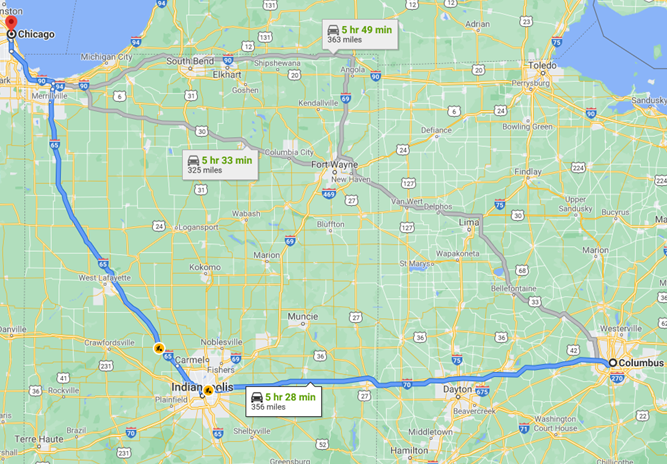
\includegraphics{ColumbusChicago.png}
%\end{image}
%
%
%Draw graphs in tikzi when possible.  Here are two.
%
%\begin{image}
%\begin{tikzpicture}
%    \begin{axis}
%        \addplot[samples=200,domain=0.01:8]{ln(x)};
%    \end{axis}
%\end{tikzpicture}
%\end{image}
%
%\begin{image}
%\begin{tikzpicture}
%    \begin{axis}[xlabel={},ylabel={},width=0.75\linewidth,
%                xmin=-5,xmax=5,
%                ymin=-5,ymax=5,
%                xtick={-4,4},
%                ytick={-4,4},
%                clip=false]
%        \addplot[soliddot] coordinates {(0,0)} node[pin=240:{Carl's house}] {};
%        \addplot[soliddot] coordinates {(2, 3)} node[pin=-30:{restaurant}] {};
%        \addplot[soliddot] coordinates {(-3, 2)} node[pin=100:{pet shop}] {};
%        \addplot[soliddot] coordinates {(-2, -4)} node[pin=150:{gas station}] {};
%        \addplot[soliddot] coordinates {(3, -3)} node[pin=120:{bar}] {};
%        \addplot[mark=none] coordinates {(5, 0)} node[above left] {east};
%        \addplot[mark=none] coordinates {(-5, 0)} node[above right] {west};
%        \addplot[mark=none] coordinates {(0, 5)} node[below right] {north};
%        \addplot[mark=none] coordinates {(0, -5)} node[above right] {south};
%    \end{axis}
%\end{tikzpicture}
%\end{image}
%
%
%You can also add Desmos interactives.  Create them in a Desmos account (I think we have an OSU one.  We should look into that!).  Save them.  Then pull the graph number out of the url.
%\begin{center}  
%\desmos{lxllnpdi6w}{800}{600}  
%\end{center}
%
%%\typeout{************************************************}
%%\typeout{Online Features}
%%\typeout{************************************************}
%
%\section{Online Features}
%
%To add a url, use the link command.
%For more about formatting in Ximera see \link[this url]{https://ximera.osu.edu/intro/gettingStarted/graphicsAndVideos/graphicsAndVideos}.
%
%
%You can also embed \link[YouTube]{https://www.youtube.com/} videos.
%\begin{center}
%\youtube{0aQpLSu2fMs}
%\end{center}
%
%
%
%
%
%\newpage
%
%%\typeout{************************************************}
%%\typeout{Overviews}
%%\typeout{************************************************}
%
%\section{Overviews}
%
%Each Unit has an overview with the organization and learning objectives
%
%\begin{overview}
%\item Generally a folder %(author if relevant)
%	\begin{enumerate}
%	\item some stuff covered in these sections
%		\textit{a subtopic} 
%		\textit{another subtopic} 
%	\item More stuff	
%	\end{enumerate}	
%\item Another Folder 
%	\begin{enumerate}	
%	\item Stuff 
%	\end{enumerate} 
%\end{overview}
%
%
%\begin{objectives}
%\item Learning Objectives Category (Course level learning objective)
%	\begin{itemize}
%	\item more specific goal
%	\item another one 
%	\end{itemize}
%\item Another Category
%	\begin{itemize}
%	\item Linear 
%	\item Parabolas 
%	\item Polynomials 
%	\end{itemize}
%\end{objectives}
%
%
%
%
%\newpage
%
%%\typeout{************************************************}
%%\typeout{Homeworks}
%%\typeout{************************************************}
%
%\section{Homework}
%Each homework problem should be it's own file.  Then the homework is put together using an exerciselist file.  See a Unit 1 folder for an example.  Be sure to keep all the same conventions, just changing the actual problem.  
%
%Some Ximera problem types are available \link[in the footnote]{https://ximera.osu.edu/intro/gettingStarted/questionAndAnswerTypes/questionAndAnswerTypes}.  We can add more here as we come across them.

\end{document}
